% --------------------------------------------------------------------------- %
% --------------------------------------------------------------------------- %
\chapter{Introduction}
\label{ch:intro}
% --------------------------------------------------------------------------- %
% --------------------------------------------------------------------------- %

The goal of particle physics it to understand the basic laws governing the
nature of matter and its interactions. Throughout the twentieth century,
particle physics experiments and theoretical work have culminated in a model
that governs the electromagnetic, weak and strong nuclear interactions, which
mediate the dynamics of the known subatomic particles. Since then, discoveries
of the bottom quark, the W and Z bosons, the top quark and the tau neutrino
have given support to this model. Because of its success in explaining a wide
variety of experimental results, this theory is regarded as the "Standard
Model" (SM).

The latest particle accelerator, the Large Hadron Collider (LHC), was built to
explore the predictions of different theories of particle physics, particularly
to provide evidence for the existence of the theorized Higgs Boson and a large
family of new particles predicted by "Supersymmetric" theories~\cite{lhcgoal}.
The LHC is a proton-proton collider built along the Franco-Swiss border
that will eventually operate at a design energy seven times larger than the
previous generation accelerator. Built to observe the high energy proton-proton
collisions delivered by the LHC, the Compact Muon Solenoid (CMS) is a
general-purpose particle detector used to investigate a wide range of physics,
including the search for the Higgs boson, extra dimensions, Supersymmetry, and
particles that make up dark matter.

The goal of this thesis is to perform one of these general searches for new
physics using the final state with two leptons with the same electric charge
that arise from the decay of gauge bosons. It uses the full dataset of 8 \TeV
collisions collected by CMS during the 2012 run and corresponds to 19.5 \fbinv
of integrated luminosity. This is a promising signature because the expected
Standard Model backgrounds are relatively rare and any new physics with this
final state would show up an excess of collision events. The results of this
thesis expand on results previously published using 10.5 \fbinv of the 2012
data~\cite{sspaper2012}. Several changes have been made with respect to this
analysis including changes to the lepton selection and expanded search regions
to achieve maximum sensitivity.

This thesis is organized into eight chapters. First, I will present
a brief review of the standard model and motivate the analysis in
Chapter~\ref{ch:intro}. An overview of the LHC followed by a discussion of
the CMS detector along with the algorithms it uses to reconstruct the decay
products of the proton-proton collisions is given in Chapter~\ref{ch:cms}. In
Chapter~\ref{ch:ss}, I present a discussion of the main sources of backgrounds
in this analysis from the Standard Model and briefly discuss other sources
of background due to algorithmic effects. The main analysis is shown in the
next four chapters with the event selection (Chapter~\ref{ch:evtsel}), the
background estimation (Chapter~\ref{ch:bkgd}), the efficiency measurements
(Chapter~\ref{ch:eff}) and finally the results (Chapter~\ref{ch:results}). The
last chapter concludes the thesis.

% --------------------------------------------------------------------------- %
% --------------------------------------------------------------------------- %
\section{Standard Model of Particle Physics}
\label{sec:intro_sm}
% --------------------------------------------------------------------------- %
% --------------------------------------------------------------------------- %

Starting with the beginning of the twentieth century, our understanding of
matter has progressed from little knowledge of the structure of matter
to a theoretical framework that predicts, to very high accuracy, many of the
observed particle interactions from experiments performed throughout the
previous century. Currently, matter and energy are best understood in terms of
the kinematics and interactions of elementary particles. The laws governing
the behavior and interaction of all known forms of matter and energy have been
reduced to a small subset of fundamental theories. The Standard Model represents
a theory that predicts the interactions of all known particles through the
electromagnetic, weak, and strong nuclear forces.

The SM has 61 elementary particles which are summarized in the
Figure~\ref{fig:intro_particles} below and fall into two
categories -- fermions and bosons~\cite{halzen}.

% --------------------------------------------------------------------------- %
\begin{figure}[tbhp]
\centering
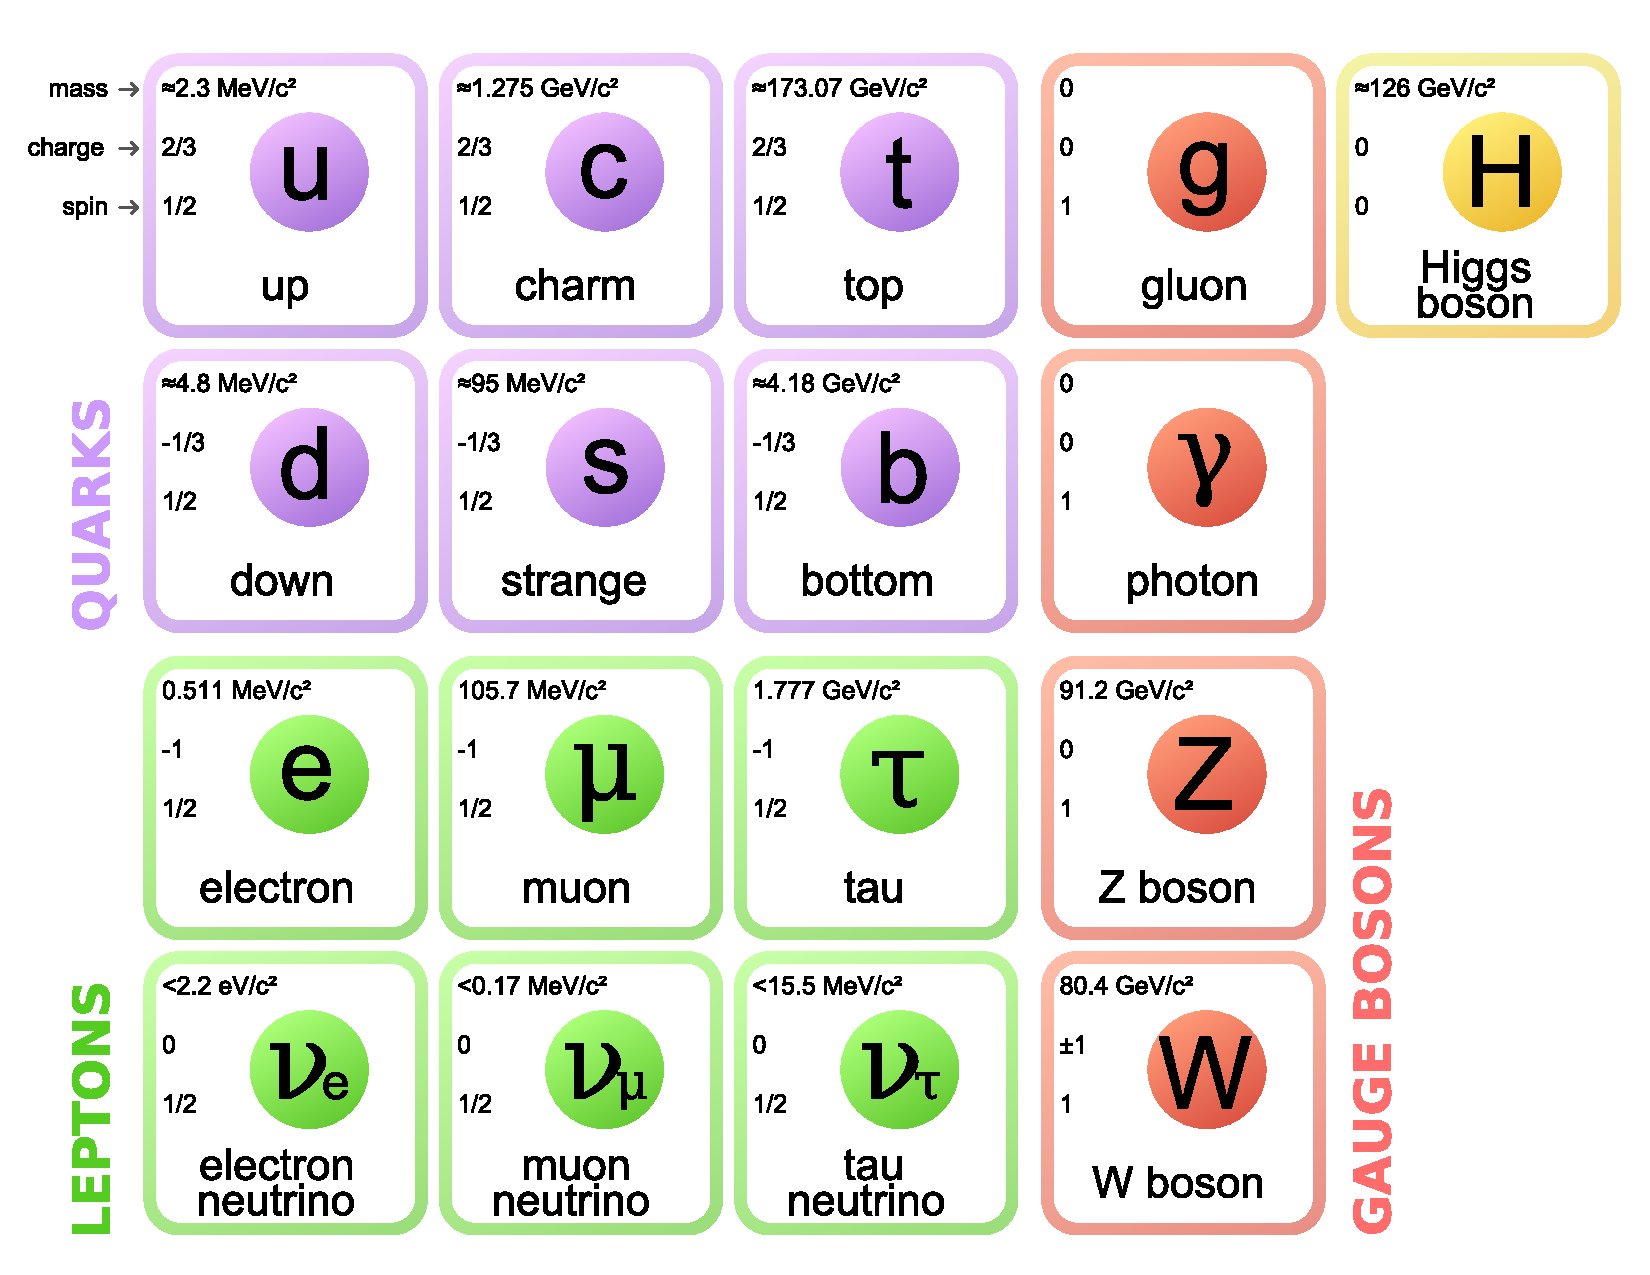
\includegraphics[width=0.8\textwidth]{particles.pdf}
\caption[The list of fundamental Standard Model particles broken down by particle type]
{\label{fig:intro_particles}
The list of fundamental Standard Model particles broken down by particle type:
quarks in purple, leptons in green, gauge bosons in red, and the Higgs boson in
yellow. The anti-quarks and anti-leptons are not shown~\cite{wikiparticles}.
}
\end{figure}
% --------------------------------------------------------------------------- %

% --------------------------------------------------------------------------- %
\subsubsection{Fermions}
\label{sec:intro_sm_fermions}
% --------------------------------------------------------------------------- %
The SM includes twelve spin-$\rm{\frac{1}{2}}$ elementary particles known as
fermions that make up all known matter in the universe. These fermions respect
the Pauli exclusion principle and each has a corresponding anti-particle. The
SM classifies the fermions according to how they interact through the quantum
numbers they carry. There are six quarks each assigned a different flavor
quantum number: up, down, charm, strange, top, and bottom. The remaining six
fermions are the leptons which are also identified by their flavor: electron,
electron neutrino, muon, muon neutrino, tau, and tau neutrino. Pairs from each
are classified and grouped together to form generations, which correspond to
particles exhibiting similar physical behavior.

The major property of the quarks is that they carry the color charge and
interact via the strong interaction. A phenomenon called color confinement
results in quarks being bound to one another, forming color neutral composite
particles called hadrons. Hadrons fall into two main categories: mesons which
are quark and antiquark bound states and baryons which are bound states of
three quarks (or three antiquarks). The familiar proton and the neutron are the
two baryons with the lowest mass. Quarks also carry electric and weak charges
and hence, they interact with all fermions via both the electromagnetic and
weak interactions.

The other main category of fermions, the leptons, do not carry color charge
and do not participate in the strong interaction. The three neutrinos do not
carry electric charge either, so they are only influenced by the weak nuclear
force. This property leads neutrinos to be notoriously difficult to detect
experimentally. However, the remaining three leptons do carry electric charge:
the electron, muon and tau all interact electromagnetically.

All 12 fermions are grouped into three generations where each member of
a generation has a greater mass than the corresponding particle in lower
generations. The first generation of quarks and leptons do not decay; hence
all ordinary matter is made up of such particles. Specifically, all atoms
consisting of electrons orbiting the nucleus which is made up of up and down
quarks. Second and third generations particles are very short lived and are
only produced in very high-energy environments (such as the LHC). Neutrinos
of all generations also do not decay and very rarely interact with matter.

% --------------------------------------------------------------------------- %
\subsubsection{Bosons}
\label{sec:intro_sm_bosons}
% --------------------------------------------------------------------------- %
In the SM, gauge bosons play the roll as the ``force carriers'' and are the
mediators of the strong, weak and electromagnetic fundamental forces or
interactions. The SM explains such forces as resulting from matter particles
exchanging these bosons, known as force mediators. At a macroscopic level, the
effect is equivalent to a force field influencing both of them; however, when
looking at the microscopic level, a gauge boson has been exchanged. The gauge
bosons of the SM all have spin-1, and as a result, they do not follow the Pauli
exclusion principle that constrains fermions and thus have no limit on their
spatial density. The different types of gauge bosons are described below:
% --------------------------------------------------------------------------- %
\begin{itemize}
\item Photons ($\gamma$) mediate the electromagnetic interaction between
charged particles. The photon is massless and is described by the subset of the
SM known as quantum electrodynamics.
\item The $W^+$, $W^-$, and Z gauge bosons mediate the weak interactions
between particles of different flavors (all quarks and leptons). They are
massive with the $W^{\pm}$ and Z bosons being 80.4 \GeVcc and 90.2 \GeVcc,
respectively~\cite{pdg}. The $W^+$ and $W^-$ bosons carry an electric charge
(indicated by the superscript) and the Z boson is electrically neutral. The
final characteristic is that the W bosons decay weakly into final states of
either two quarks or two leptons. In the case of the two quark final state, one
quark must be a up-type quark (up, charm) and the other a down type anti-quark
(down, strange, or bottom). The W does not decay via a top quark due to
kinematic constraints imposed by the much more massive top quark. In the case
where the W boson decays to a lepton pair, one lepton must be a charged lepton
(electron, muon, or tau) and the other must be a neutrino (electron neutrino,
muon neutrino, or tau neutrino). Finally, the Z boson must decay to a fermion
and its anti-particle. For example $\Zlplm$ or $Z \to q\bar{q}$ where $q$
represent a quark, $\bar{q}$ represents an antiquark, and $\ell$ represents a
charged lepton.
\item The eight gluons (g) mediate the strong interactions between color
charged particles (the quarks). Gluons are massless. The eightfold multiplicity
of gluons is labeled by a combination of color and anticolor charge, and
because gluons themselves carry a color charge, they can interact
among themselves. The gluons and their interactions are described by the theory
of chromodynamics.
\end{itemize}

% --------------------------------------------------------------------------- %
The final boson in the SM is the Higgs boson and is a key building block
in the underlying structure of the theory. It has no intrinsic spin
(scalar), is massive at 125.7 \GeVcc~\cite{higgstwiki}, and plays a unique roll by
explaining why other elementary particles, except the photon and gluon, are
massive~\cite{discovery}. In particular, they explain why the photon has no
mass, while the W and Z bosons do. Also, in electroweak theory, the Higgs
boson generates the masses of the leptons and quarks. Finally, as the Higgs is
massive, it must interact with itself.

The following Figure~\ref{fig:intro_int} shows a summary of all the allowed
interaction between particle types in the Standard Model.
% --------------------------------------------------------------------------- %
\begin{figure}[!hbt]
\centering
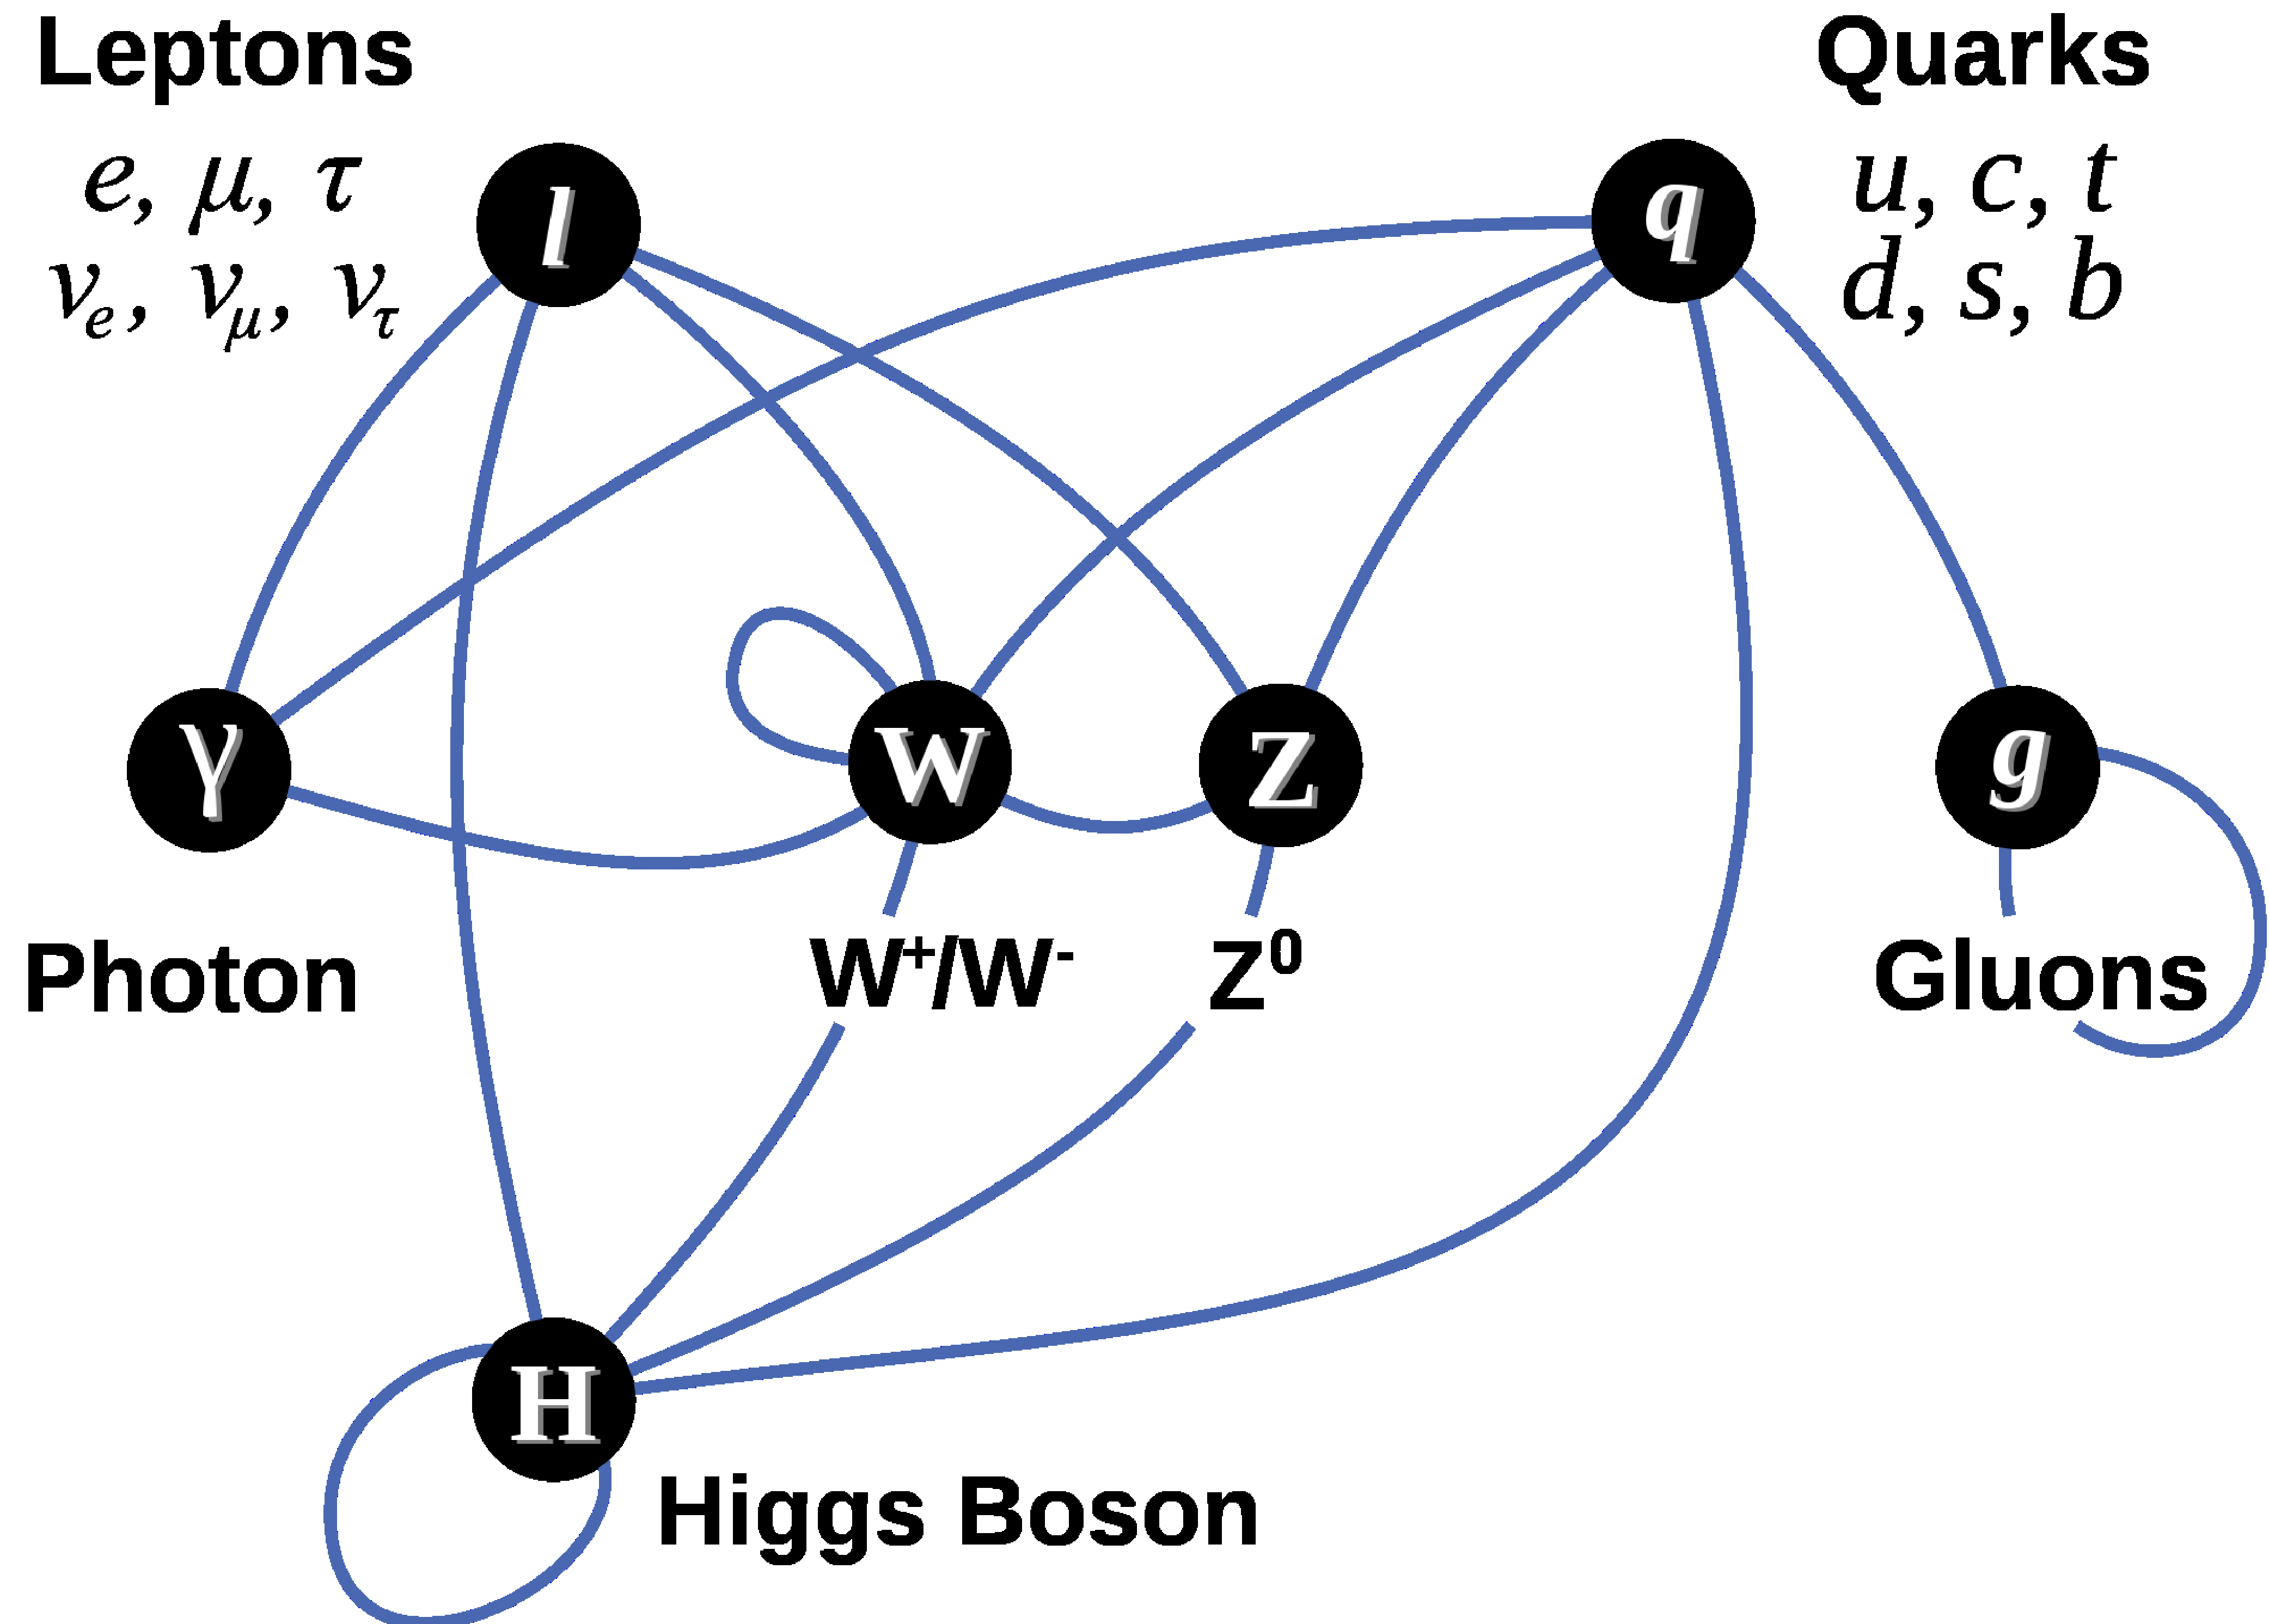
\includegraphics[width=0.6\textwidth]{interactions.pdf}
\caption[A summary of the allowed interactions between particle types in the Standard Model]
{\label{fig:intro_int}
A summary of the allowed interactions between particle types in the
Standard Model. A line connecting two particles indicates coupling occurs
between those particles. A line from one particle to itself indicates
that this particular particle self-couples~\cite{wikiinteractions}.
}
\end{figure}
% --------------------------------------------------------------------------- %

% --------------------------------------------------------------------------- %
\subsubsection{Known deficiencies of the SM}
\label{sec:intro_sm_issues}
% --------------------------------------------------------------------------- %
The Standard Model is not considered a complete theory. Some of the major
issues are outlined below:
% --------------------------------------------------------------------------- %
\begin{itemize}
\item The SM does not provide a mechanism to explain gravitation. Attempts have
been made to find a quantum theory of gravity that is also consistent with
general relativity; however, these theories break down before reaching the
Planck scale and therefore are not satisfactory.
\item The SM is considered {\it ad hoc} and inelegant since it requires many
numerical constants that seem arbitrary and unrelated.
\item The Higgs mechanism gives rise to the hierarchy problem if any new
symmetries or particle interactions are present at a high energy scale. In
order for the weak scale to be much smaller than the Planck scale, severe fine
tuning of the SM parameters is required.
\end{itemize}
% --------------------------------------------------------------------------- %
Also there are many questions in physics that are unanswered by the SM. Some of
these issues include:
% --------------------------------------------------------------------------- %
\begin{itemize}
\item Why do particle masses and coupling constants have the values that we measure?
\item Why are there three generations of particles?
\item Why is there more matter than antimatter observed in the universe?
\item Where does dark matter fit into the model?
\item Where does dark energy fit into the model?
\end{itemize}
% --------------------------------------------------------------------------- %
Clearly the SM does not provide the final explanation of all the observed
interactions in nature.

% --------------------------------------------------------------------------- %
% --------------------------------------------------------------------------- %
\section{Proton-Proton Collisions}
\label {sec:intro_collider}
% --------------------------------------------------------------------------- %
% --------------------------------------------------------------------------- %
To probe some of the unanswered question from the SM posed in the previous
Section (Section~\ref{sec:intro_sm}), protons are collided at high energy and
their debris is studied in detail. In particle physics, the probability for an
interaction to occur is given by the cross section ($\sigma$), which represents
the effective area presented by the target to an incoming particle. The units
for cross section are given in terms of a barn (b) where $1\ \barn = 10^{-24}\
\rm{\cm^2}$. The total number of interactions is given by the relation
% --------------------------------------------------------------------------- %
\begin{equation}
    N = \Lumi \cdot \sigma,
\end{equation}
% --------------------------------------------------------------------------- %
where $N$ is the number of interactions occurring in an instantaneous
luminosity of \lumi for a process with an interaction cross section $\sigma$.
The total amount of data collected is traditionally reported as the total
integrated luminosity reported by the above relation. The integrated luminosity
has units of inverse barns (\binv); however, due to the inconvenience of the
scale of this unit, it is customary to report the units in either inverse
picobarns (\pbinv = $10^{12}$ \binv) or inverse femtobarns (\fbinv = $10^{15}$
\binv).

The difficulty of producing and storing antiprotons led to the decision to use
proton-proton (pp) collisions at the LHC~\cite{lhcmachine}. The cross section
for a typical pp collision $\approx 100$ mb~\cite{qcdprimer}. This however,
combines both elastic collisions, where the two colliding protons remain whole,
and inelastic collisions, where the proton breaks apart into its constituent
quarks or gluons (partons). For inelastic collisions, QCD does not allow for
a quantitative calculation of the exact kinematics of the partons that make
up the proton. Instead, one has to appeal to a series of experiments designed
to create an empirical model of the kinematic distributions of these partons.
This is done with deep inelastic scattering experiments where a high energy
electron is collided with the proton~\cite{halzen}. By measuring the resulting
momentum and angular distributions of the proton's debris, one can determine of
the fraction of energy carried by the partons which make up the proton. As an
example, Figure \ref{fig:intro_partons} shows the fraction of energy carried by
gluons and quarks for two different energy protons. Notice that while the up
and down quarks and the gluons are the dominant high momentum carriers, there
is still significant momentum from the other partons (sea quarks).

% --------------------------------------------------------------------------- %
\begin{figure}[tbhp]
\centering
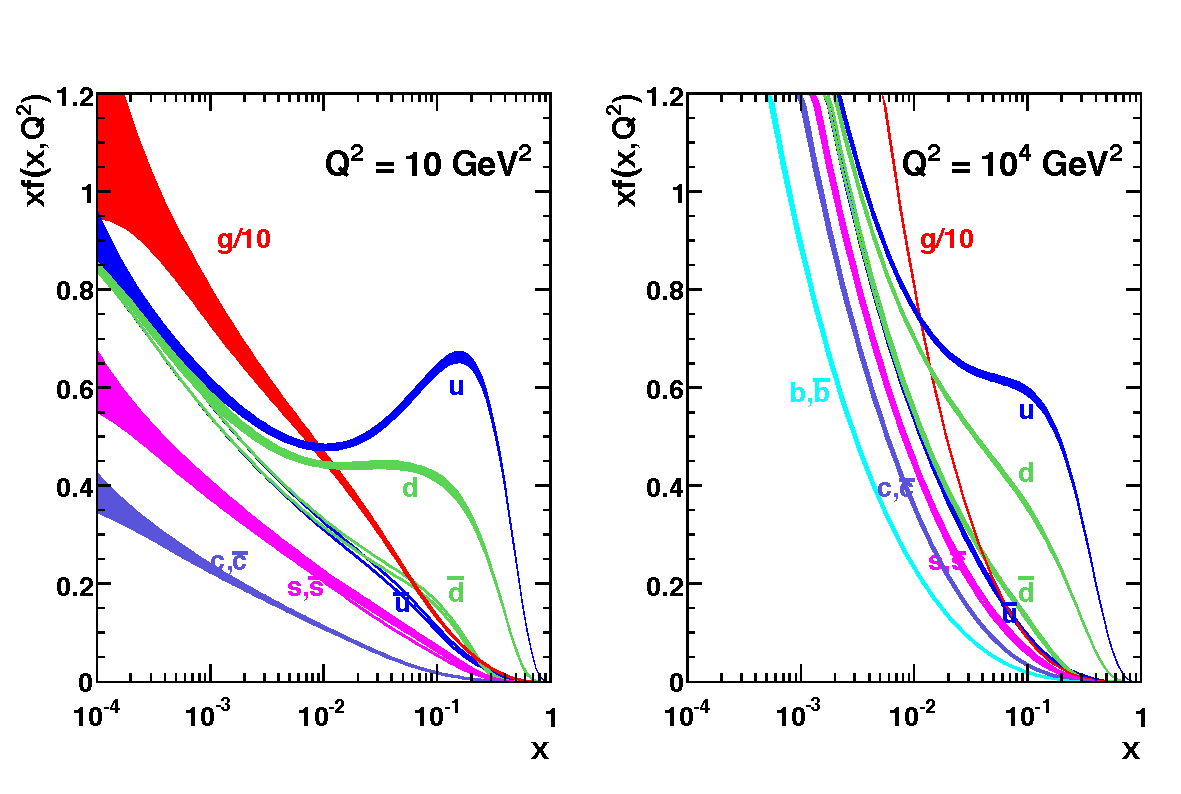
\includegraphics[width=0.8\textwidth]{partons}
\caption[Parton distribution functions for protons at $Q^2=10~\GeV^2$ and $Q^2=10000~\GeV^2$] 
{\label{fig:intro_partons}
The parton distribution functions and their associated error
for a proton at a momentum transfer scale of $Q^2=10~\GeV^2$ (left) and
$Q^2=10000~\GeV^2$ (right) as a function of $x$, the fraction of the proton's
momentum carried by the parton~\cite{partons}.
}
\end{figure}
% --------------------------------------------------------------------------- %

% --------------------------------------------------------------------------- %
% --------------------------------------------------------------------------- %
\section{Motivation for Same-Sign Dilepton Signature}
\label {sec:intro_ss}
% --------------------------------------------------------------------------- %
% --------------------------------------------------------------------------- %
One of the purposes of the LHC and CMS is to search for physics beyond
the Standard Model (BSM). As mentioned in Section~\ref{sec:intro_sm},
astrophysical evidence for dark matter suggests that the SM is incomplete.
Although direct detection experiments have yet to make an observation,
indirect measurements are pointing to dark matter being related to the weak
interaction~\cite{darkmatter,baer}. It is clear that the SM is not the full
story describing particle interactions. The physics analysis discussed in this
thesis attempts to take advantage of the strengths in lepton reconstruction
to search for previously unobserved physics.

Figure~\ref{fig:intro_smxsec} shows the production cross section for a number of SM
processes as a function of the center-of-mass energy of the colliding beams.
% --------------------------------------------------------------------------- %
\begin{figure}[tbhp]
\centering
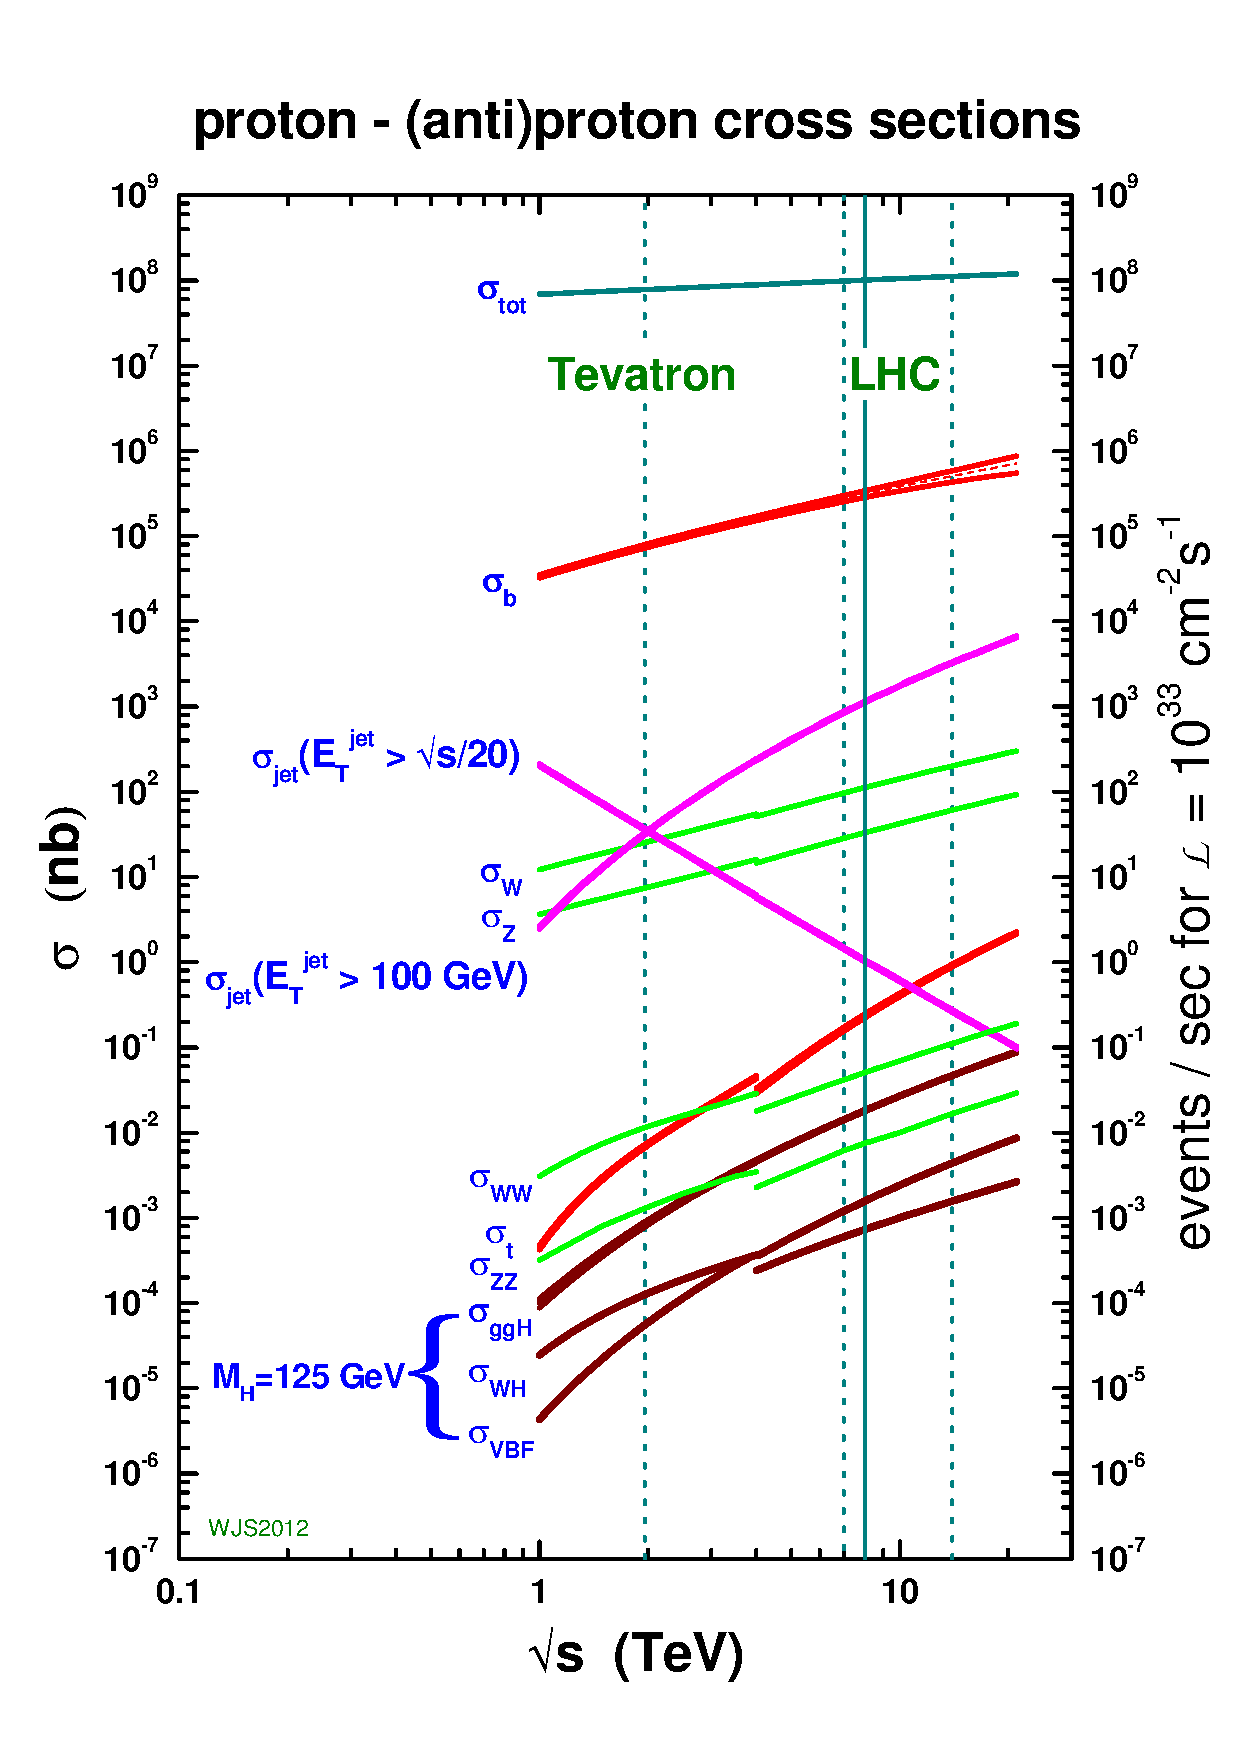
\includegraphics[width=0.8\textwidth]{smxsec}
\caption[Cross sections for some Standard Model process vs center-of-mass energy] 
{\label{fig:intro_smxsec}
Cross sections for some Standard Model processes vs center-of-mass energy.
The cross sections of SM process giving final state leptons are many orders of
magnitude smaller than QCD cross sections. From~\cite{smxsec}.
}
\end{figure}
% --------------------------------------------------------------------------- %
Comparing the relative size of the total inelastic collisions cross section,
contaminated by QCD processes, with that for W boson production, it is apparent
that these electroweak processes are rare in the SM. Subsequent leptonic
decays of the W boson occurs at the rate of $\approx 30\%$, making leptons
originating from a W boson even more rare. Sources of dilepton final states
are significantly more rare with the dominant source being \Zlplm. Additional
sources of dileptons include \ttbar, \WW, \WZ, and \ZZ production, all
with smaller production cross sections. Most of the dilepton pairs from these
have opposite electric charge (+/-). Since these lepton are both prompt and
relatively isolated, they provide an extremely clean experimental signature
in the detector since they are simpler to reconstruct with smaller rates of
mis-measurement. The combined effect is much smaller backgrounds for searches
in dilepton final states, particularly same-sign dilepton final states ({+}{+}
or {-}{-}), compared to single lepton and fully hadronic analyses.

From the above discussion, it is clear that a signature with two prompt and
isolated leptons with the same electric charge (same-signed dileptons) is a
rare occurrence in the SM relative to other processes. As a result, searches
for anomalous production of same-sign dileptons can be very sensitive to new
physics contributions. These include
% --------------------------------------------------------------------------- %
\begin{itemize}
\item supersymmetry (SUSY) \cite{ss::barnett,ss:baer,ss:guchait},
\item universal extra dimensions \cite{ss:cheng}
\item pair production of $T_{5/3}$ particles (fermionic parters of the top quark) \cite{ss:contino}, 
\item heavy Majorana neutrinos \cite{ss:almeida},
\item and same-sign top pair production \cite{ss::sstop}.
\end{itemize}
% --------------------------------------------------------------------------- %
New physics signatures with large cross sections are likely to be produced
by strong interactions, and we thus expect significant hadronic activity in
conjunction with the two leptons. Additionally, SUSY models with R-parity
conservation and astrophysical evidence for dark matter suggest considering
final states with undetectable particles that leads to a significant amount
of missing transverse energy (\met)~\cite{AMS,Bertone:2004pz}. With the above
considerations, in this analysis, we search for new physics with events
containing:
% --------------------------------------------------------------------------- %
\begin{itemize}
\item same-sign dileptons (electrons and muons), 
\item hadronic jets (with and without b-tagging), 
\item and accompanying missing transverse energy.
\end{itemize}
% --------------------------------------------------------------------------- %
The exact event selection will be discussed in Chapter~\ref{ch:evtsel}.

The basic idea is to count the number of observed collision events that have
the above signature and compare this to the number of events that were expected
assuming the SM only. This comparison is done using statistical techniques
to be discussed in Section \ref{sec:results_int}. If there is a significant
excess of events above your expected SM background, then this gives evidence
that new physics exists beyond the SM. It is important to get the most accurate
background prediction possible to ensure maximum sensitivity to an anomalous
excess of events. The specific details of the background estimation techniques
can be found in the following chapters. Finally, in Chapter \ref{ch:results},
we show the results of this search along with some interpretations with respect
to some selected new physics models.
